\subsection{Análisis y Administración de Riesgos}

El proyecto enfrenta diversos tipos de riesgos: técnicos (dificultades en integración con pasarelas de pago, limitaciones de APIs, problemas de rendimiento del SDK), organizacionales (cambios en disponibilidad de integrantes, conflictos de prioridades con otros proyectos académicos) y académicos (cambios en criterios de evaluación, retrasos en retroalimentación del director). Para administrar estos riesgos de manera sistemática, el equipo ejecuta un proceso continuo de identificación, valoración y mitigación a lo largo de todo el proyecto.

En la reunión de planificación de cada ciclo de dos semanas, el equipo participa en una sesión de lluvia de ideas (brainstorming) de 30 minutos para identificar nuevos riesgos o cambios en riesgos ya existentes. Se consideran riesgos de todas las categorías mencionadas. El Coordinador documenta todos los riesgos propuestos en Notion sin aplicar ningún filtro inicial; en esta fase no hay criterio, solo se recopilan todas las preocupaciones del equipo. Para cada riesgo identificado, el equipo estima dos variables: probabilidad de ocurrencia (baja: <20\%, media: 20-60\%, alta: >60\%) e impacto esperado en caso de que el riesgo se concrete (bajo: retraso <3 días, medio: retraso 3-7 días, alto: retraso >7 días o cambio de alcance mayor). La prioridad del riesgo se calcula multiplicando probabilidad × impacto, y se clasifican riesgos en tres categorías: verde (prioridad <0.2, monitoreo pasivo), amarillo (0.2-0.6, requiere plan de acción), y rojo (>0.6, requiere escalada inmediata al director). Este análisis completo se registra en el Anexo B del proyecto.

En cada reunión de sincronización (jueves), se revisan los riesgos de categoría amarillo y rojo, actualizando su estado y verificando que las acciones de mitigación se estén ejecutando según lo planeado. La Líder evaluación y documentación prepara un sumario quincenal de cambios en riesgos (nuevos identificados, riesgos que han desaparecido, cambios de prioridad) que se comparte con el director del proyecto. Riesgos nuevos pueden ser propuestos en cualquier momento por cualquier integrante; se añaden inmediatamente a Notion y se evalúan en la próxima reunión de planificación. Para cada riesgo de categoría rojo o amarillo, el equipo define acciones específicas de prevención (actividades para que el riesgo no ocurra) y mitigación (cómo responder si el riesgo sí ocurre). Por ejemplo, para el riesgo técnico de "dificultad en integración con pasarelas", la prevención es realizar pruebas exploratorias tempranas con APIs de sandbox, y la mitigación es diseñar adaptadores específicos si se identifica incompatibilidad. Para el riesgo organizacional de "cambio de disponibilidad de integrantes", la prevención es mantener documentación exhaustiva de decisiones técnicas en GitHub y Google Drive, y la mitigación es asignar responsables alternos para funciones críticas. Cada acción de mitigación tiene un responsable asignado, un plazo de inicio y una descripción de recursos necesarios.

\begin{figure}[H]
  \centering
  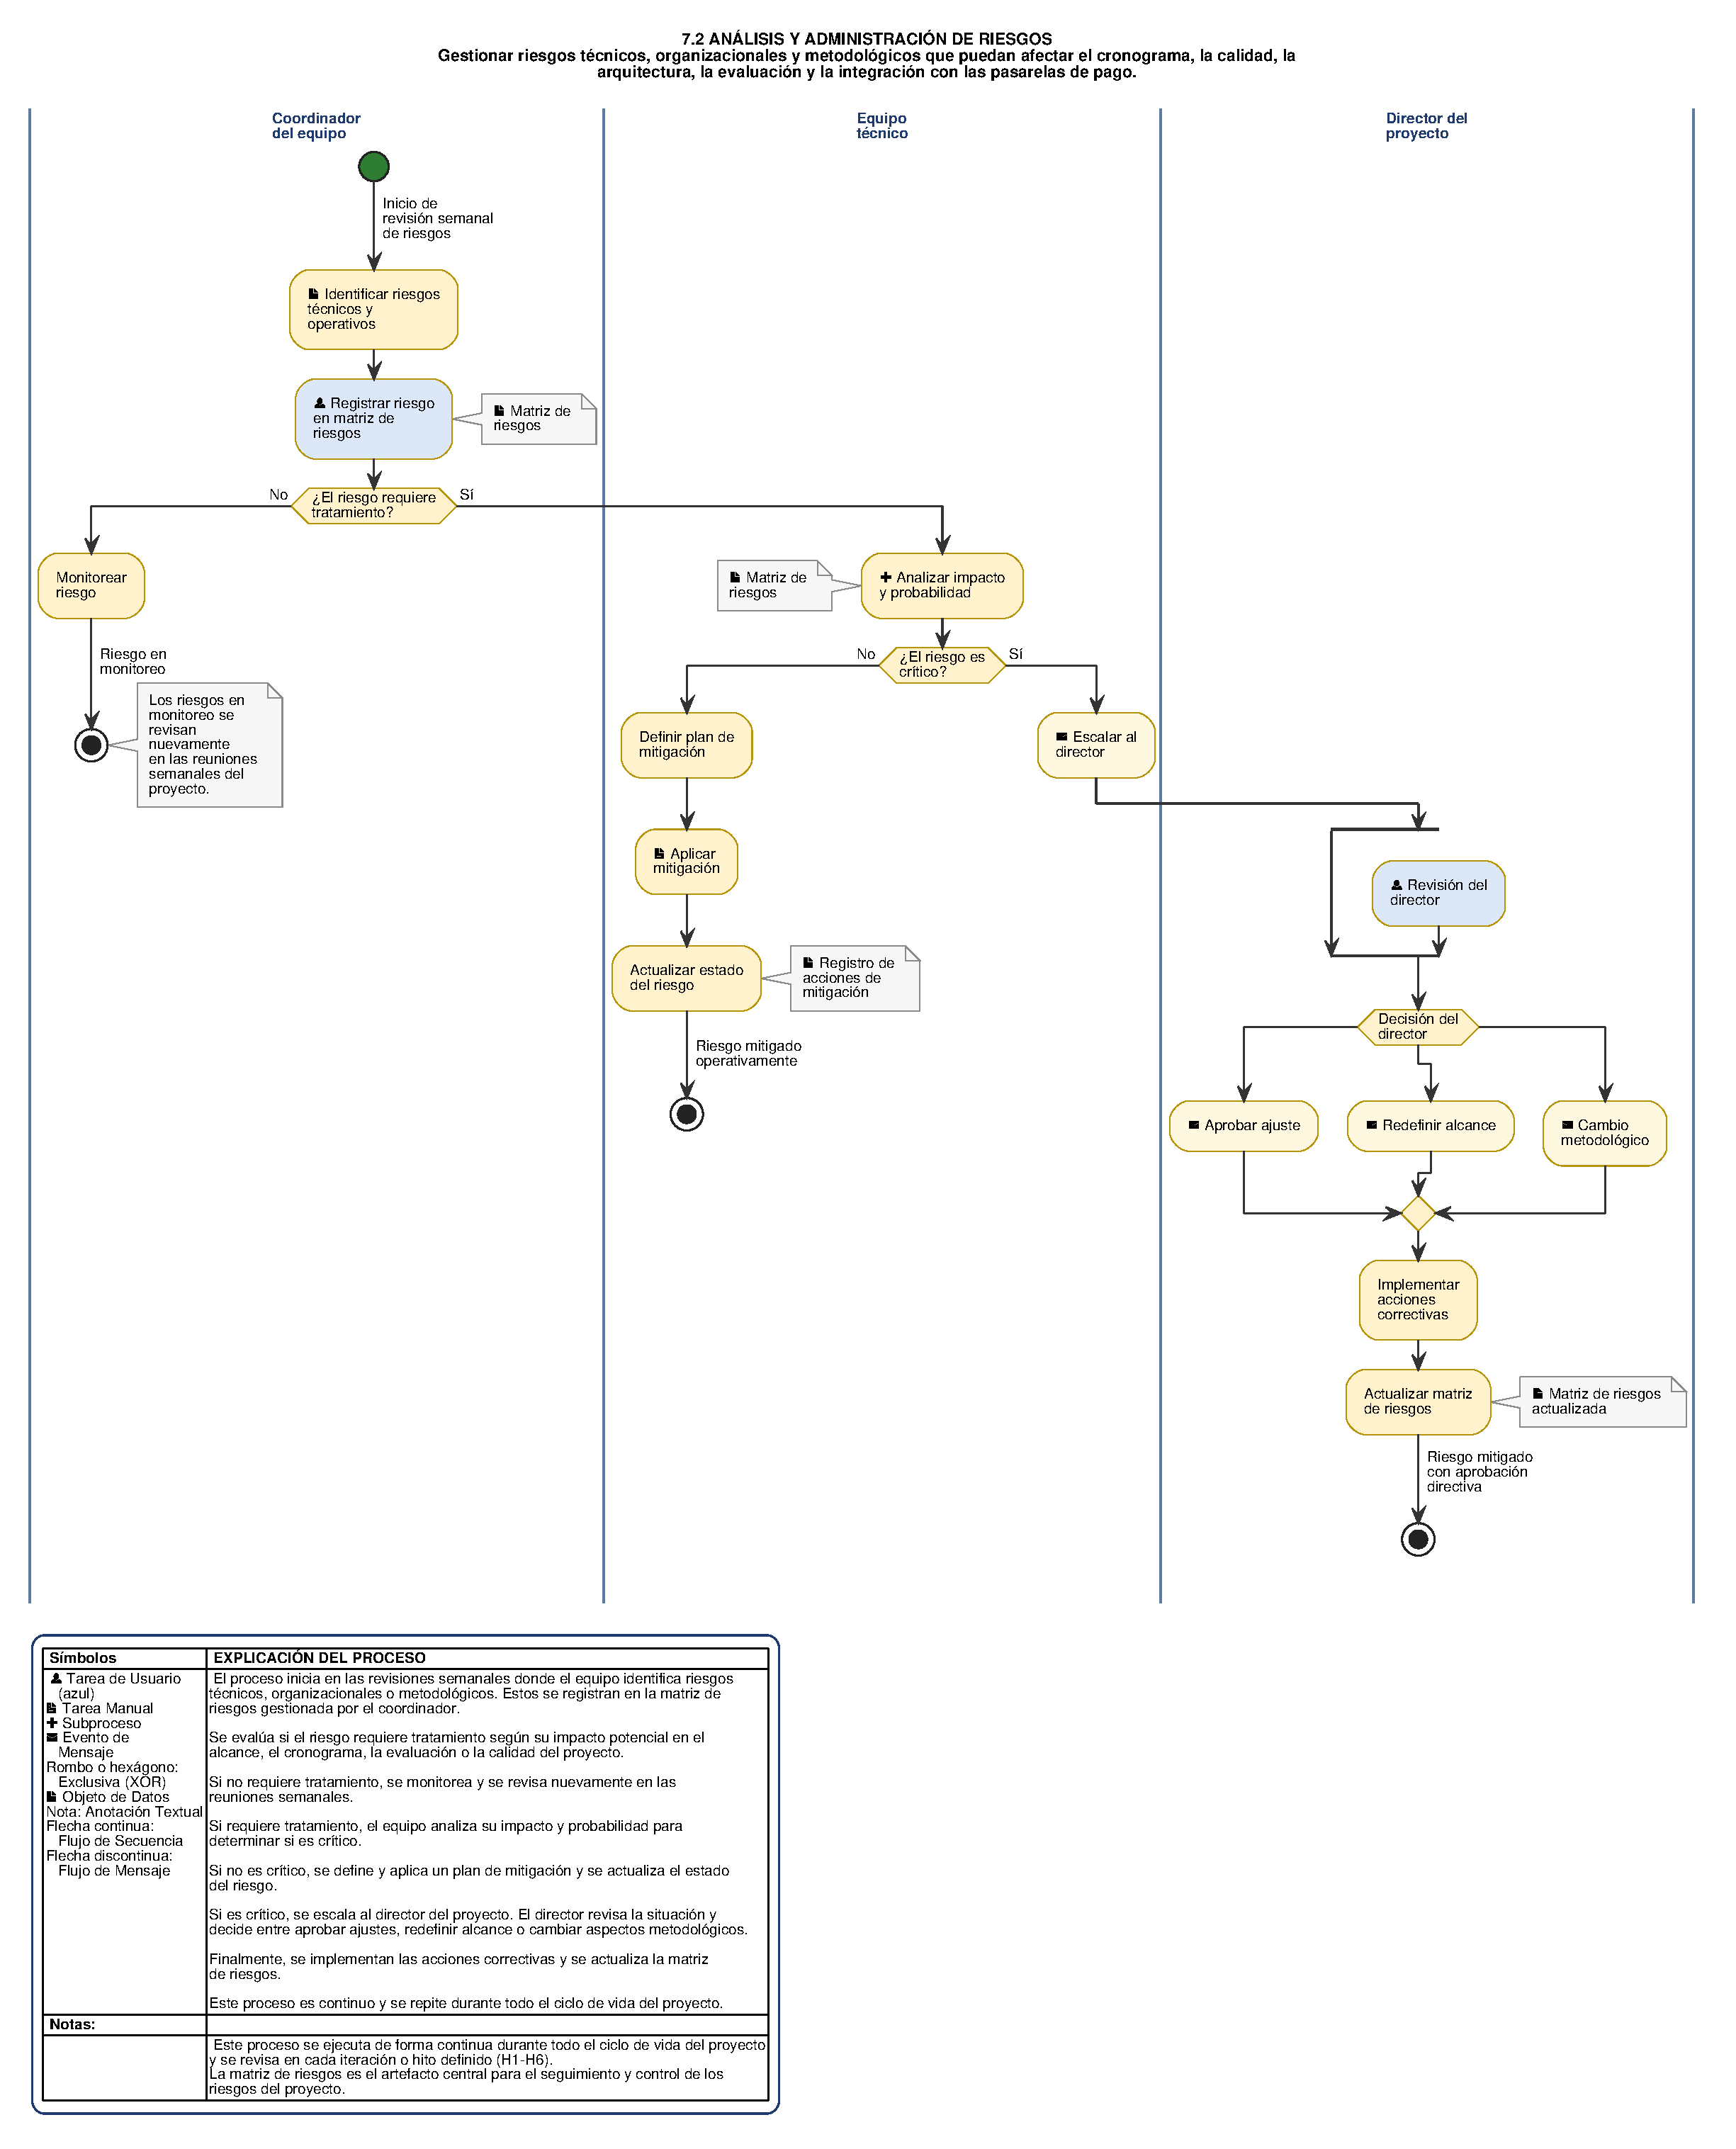
\includegraphics[width=\textwidth]{figuras/06-bpmn-riesgos}
  \caption{Diagrama BPMN para administración de riesgos}
  \label{fig:bpmn-riesgos}
\end{figure}
